\documentclass{article} % for short documents
%\documentclass{report} % for longer documents

\usepackage{minted}

%% Defining the language for the document
\usepackage[english]{babel}
\usepackage[english]{isodate}

\usepackage{imta_core}
\usepackage{imta_extra}
\usepackage{epigraph}
\usepackage{graphicx}
\usepackage{wrapfig}
\usepackage{alertmessage}
\usepackage{hyperref}
\usepackage{xcolor}


%% Addtionnal packages can be loaded here
% \usepackage{biblatex} % for a complete and flexible bibliography


\cleanlookdateon % formats date according to the loaded language from now on

%% General informations
\author{\\ Alexandre ALLANI \\
	Adrien CLOTTEAU }
%\imtaAuthorShort{<author's initials>}
%\imtaSuperviser{<superviser>}
\date{\noexpand\today} % automatically print today's date, can be redefined using \date{<date>}
\title{Rapport projet S5}
\subtitle{Challenge Total}
%\imtaVersion{<version>}

%Add extra other companies' logo
%If needed, options can be passed to the underlying \includegraphics by calling \imtaAddPartnerLogo[<options>]{<path>}
%\imtaAddPartnerLogo{<logo_path>}


\imtaSetIMTStyle % Sets font and headers/footers according to the IMT Atlantue style guidelines

%%%%%%%%%%%%%%%%%%%%%%%%%%%%%%% 
%%%%%%%%%% BEGINNING %%%%%%%%%% 
\begin{document}
	
	% front cover
\imtaMaketitlepage
\tableofcontents
\newpage

\section{Introduction}
\alertinfo{Vous trouverez l'ensemble de ce qui a été fait en suivant le lien ci-dessous. \url{https://github.com/Syndorik/ChallengeTotal}. 
}
En suivant le lien Github, vous trouverez: 
\begin{itemize}
	\item Challenge-Total-Overlook-of-the-data.ipynb : Jupyter Notebook sur la visualisation des données.
	\item Data-Engineering-and\_Modeling.ipynb : Jupyter Notebook sur la préparation des données et la modélisation.
	\item Time\_series.ipynb : Jupyter Notebook sur la modelisation avec les Time Series.
\end{itemize}
\section{Contexte}
\newpage
\section{Visualisation des données}
\alertinfo{Le code lié à cette partie est disponible sur le lien suivant \url{https://github.com/Syndorik/ChallengeTotal/blob/master/Challenge-Total-Overlook-of-the-data.ipynb}. 
}
\newpage
\section{Préparation des données (Data Engineering)}
\alertinfo{Le code lié à cette partie est disponible sur le lien suivant \url{https://github.com/Syndorik/ChallengeTotal/blob/master/Data-Engineering-and_Modeling.ipynb}. 
}
Dans cette partie, nous allons présenter la préparation des données afin qu'elles obtiennent la forme que nous avons utilisé dans nos dernières modélisations. En suivant la méthodologie CRISP, cette préparation des données est le fruit de plusieurs tests/modélisation. Nous ne présenterons que les résultats fructueux, qui ont mené à une amélioration du modèle.
\subparagraph{Modification du jeu de données}
Le jeu de données étant français et l'interpréteur utilisé étant sous le format anglo-saxon, les valeurs numériques (telles que la température, la nébulosité etc.) étaient considérées comme des chaînes de caractère à cause de la virgule. Nous avons donc remplacé les "," par des "." pour pallier à ce problème.\\
Par ailleurs, le jeu de données ne contenant aucune valeur non acquises (NA values), il n'y a pas eu de pré-traitement à réaliser.

\subsection{Segmentation temporelle}
\subsubsection{Distinction des vacances}
L'une des premières améliorations effectuées au niveau des données est la segmentation du jeu de données en périodes de "vacances" et en périodes de "travail". En effet, il est important de modéliser cette saisonnalité car les ventes sont très différentes pendant et hors des périodes de vacances. 
\begin{figure}[!h]
	\centering
	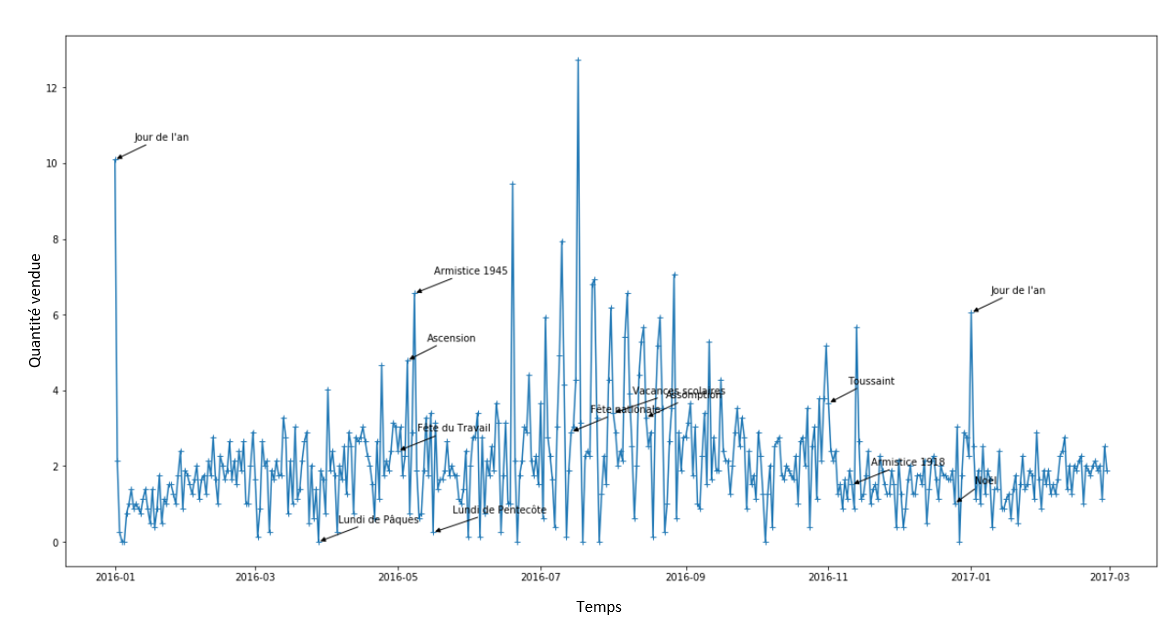
\includegraphics[keepaspectratio = true,scale=0.65]{varvente.png}
	\caption{Ventes de baguettes au cours de la période}
	\label{bbg}
\end{figure}
Le graphique ci-dessus, \textbf{Figure ~\ref{bbg}} représente les ventes des baguettes sur les deux stations durant la période couverte par le jeu de données. Les baguettes sont les produits les plus vendus, tous produits confondus. Nous pouvons observer que les ventes lors des jours fériés et périodes de vacances sont beaucoup plus élevées. En particulier, les grandes vacances sont plus sujettes à de fortes variations.\\
Ces observations sont logiques, les périodes de vacances correspondent aux périodes de départs. Les familles vont en général s'arrêter et consommer plus dans les stations-service, ainsi la quantité de produits vendus est beaucoup plus grande.\\
Segmenter l'année permet de mettre en évidence les périodes où les ventes sont très variables par rapport à la moyenne et donc permet d'affiner notre modèle. En se basant sur les \href{https://vacances-scolaires.education/annee-2015-2016.php}{\underline{\textbf{\textcolor[rgb]{0,0,1}{vacances 2015-2016}}}} et les \href{https://vacances-scolaires.education/annee-2016-2017.php}{\underline{\textbf{\textcolor[rgb]{0,0,1}{vacances 2016-2017}}}}, nous avons pu segmenter la période selon les vacances scolaires et les zones de départ en créant une nouvelle variable "holidays".
\begin{figure}[!h]
	\centering
	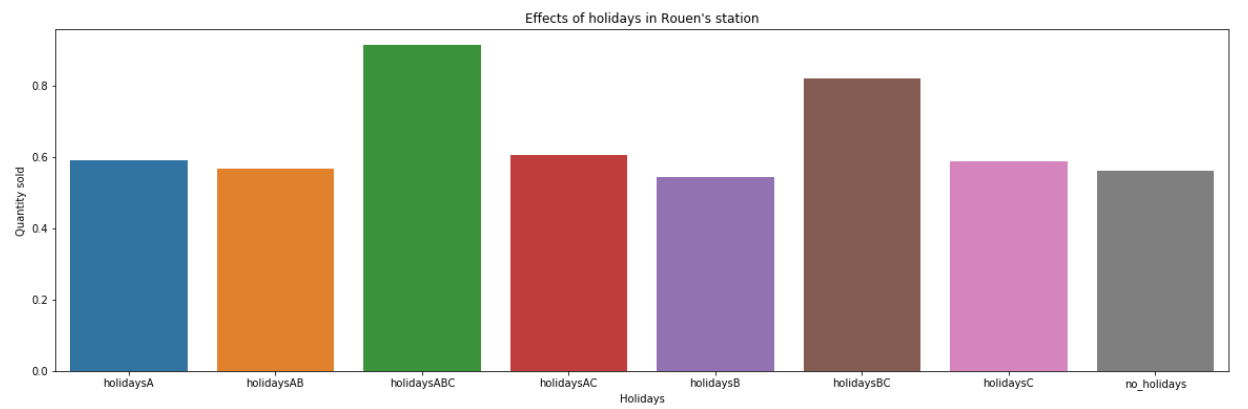
\includegraphics[keepaspectratio = true,scale=0.65]{saleholiday.png}
	\caption{Ventes cumulées par semaine selon la journée}
	\label{fig:salehol}
\end{figure}
~\\
Après création de ces variables, nous pouvons comparer les ventes moyennes entre les différentes périodes de vacances grâce à la \textbf{Figure ~\ref{fig:salehol}}. Il apparait qu'il y a une réelle différence lorsque toutes les zones (A, B, C) sont en vacances par rapport à seulement les zones (B,C). Dans les autres cas, il n'y a pas beaucoup de différences avec les périodes de travail. Cela s'explique par le fait que les stations situées à Rouen sont en zone B, et la plupart des voyageurs se dirigeant vers Rouen doivent passer par Paris (zone C). Ainsi lorsque les deux zones sont en vacances en même temps, il y a bien plus d'aller-retour qu'en période normale. Nous choisissons de garder la discrimination entre les vacances pour les trois zones (A,B,C), les vacances pour les zones B et C, et finalement les périodes de "travail".
\subsubsection{Distinction des dates de départs}
Nous pouvons voir sur la \textbf{Figure ~\ref{bbg}} que les premières journées et dernières journées de vacances sont particulièrement hautes en terme de quantités vendues. Ce sont, en effet, des journées où beaucoup de familles sont sur les routes, ainsi il y a mécaniquement plus de ventes qui sont effectuées.\\
Il est donc intéressant de discriminer ces journées afin de mieux les modéliser. Pour cela nous avons créé une nouvelle variable "departure"  qui segmente le jeu de données selon les dates de départ.

\subsubsection{Segmentation de la période selon les journées et mois}
Dans l'optique d'exploiter au maximum les saisonnalités des ventes, nous avons continué à travailler sur les dates. Comme nous pouvons le remarquer sur la \textbf{Figure ~\ref{bbg}}, les ventes atteignent un maximum local de manière périodique environ tous les 7 jours. Il y a une périodicité remarquable au niveau de la semaine. En effet, le trajet Paris-Rouen ne dure que 2 heures, il est envisageable que certaines personnes fassent l'aller-retour chaque semaine pour rentrer le week-end, et donc s'arrêtent aux deux stations-service.\\
\begin{figure}[!h]
	\centering
	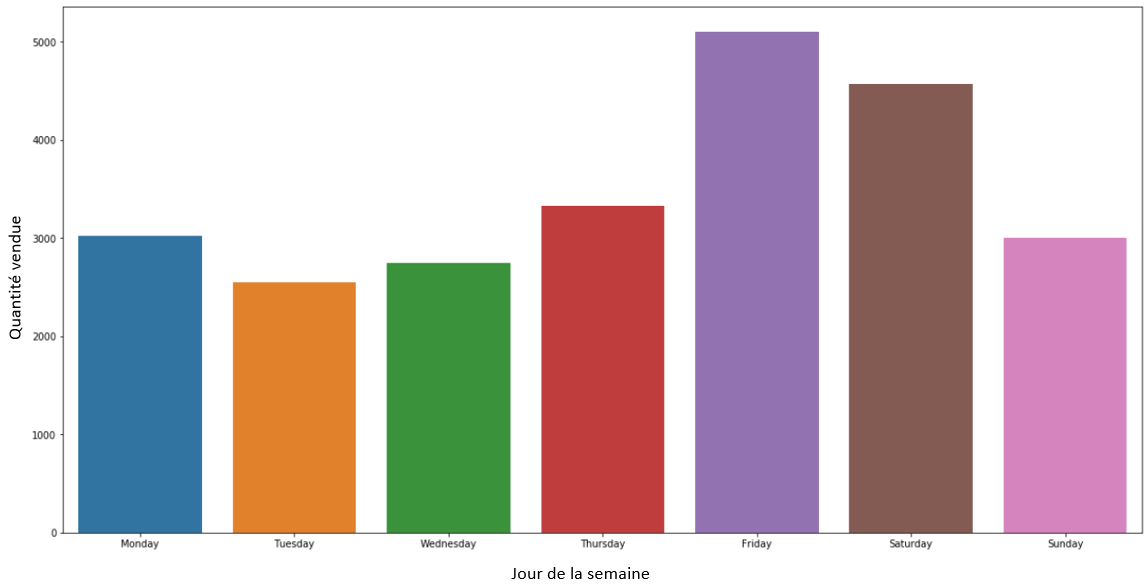
\includegraphics[keepaspectratio = true,scale=0.65]{vente_week.png}
	\caption{Ventes cumulées par semaine selon la journée}
	\label{bb1}
\end{figure}
~\\
La \textbf{Figure ~\ref{bb1}} représente les ventes cumulées sur la période du jeu de données en fonction des jours de la semaine. Elle met en évidence cette périodicité. Les ventes des journées du Vendredi et Samedi sont bien au-dessus des autres jours de la semaine. De manière générale, les ventes sont faibles pendant la semaine et hautes pendant le week-end. C'est pourquoi nous avons différencié chaque jour de la semaine dans notre jeu de données.\\
\subsubsection{Suppression de la colonne date}
Une fois ces transformations réalisées, nous supprimons la colonne date. En effet pour les modèles que nous allons utiliser (excepté pour les Time Series), garder les dates va entraîner du sur-apprentissage. Les modèles vont apprendre sur la date exacte (jour-mois-année), sachant que ces dates sont passées, cela va entraîner une grande erreur.\\
Il est à noter que toutes ces segmentations temporelles ont pour but d'affiner le modèle, et retirer le plus d'information de la variable \textit{date}. Cependant pour le modèle basé sur les Time Series, ces segmentations ne seront pas conservées, car incompatibles avec le modèle. Nous expliciterons ce sujet dans la \textbf{section ~\ref{sec:tm}}

\subsection{Influence des catégories}
Nous voulions savoir si la distinction par catégorie était utile, sachant qu'il y a inclusion des catégories : $cat6 \subset cat5 \subset cat4$. La \textbf{Figure ~\ref{cat5p1} et ~\ref{cat5p2} } représente les ventes en fonction de la catégorie 5 pendant la période.\\ 
\begin{figure}[!h]
	\centering
	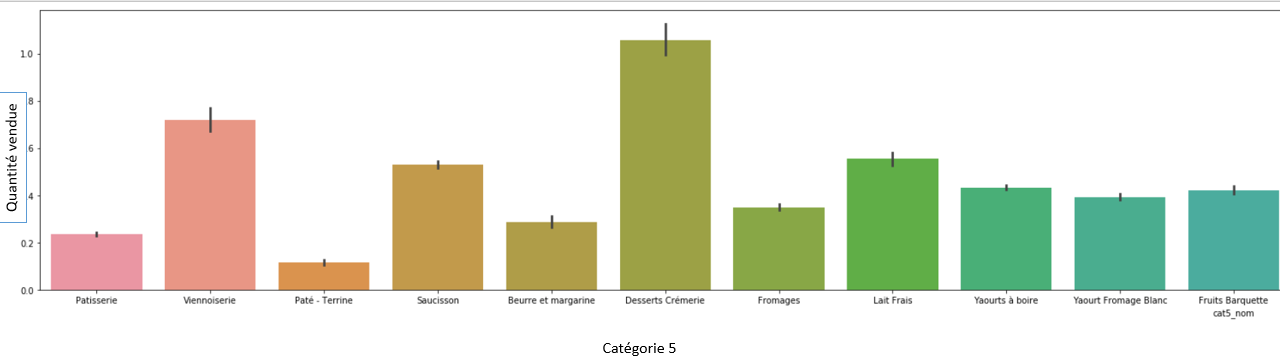
\includegraphics[keepaspectratio = true,scale=0.65]{categorie5part1.png}
	\caption{Ventes cumulées en fonction de la catégorie 5 (partie 1)}
	\label{fig:cat5p1}
\end{figure}
~\\
Il est clair qu'il y a une différence de ventes en fonction de la catégorie. La catégorie \textit{Sandwich} ou encore \textit{Dessert Crémerie} domine, tandis que la catégorie \textit{pâté} et \textit{autre charcuterie} font de faibles ventes. Cependant comme  on peut le voir sur la \textbf{Figure ~\ref{bb3}} (Annexe ~\ref{sec:catprod}), il y a peu de différence entre les sous-catégories, en particulier entre la catégorie 5 et 6 qui paraissent être presque les mêmes. Cela s'explique par l'inclusion des catégories.\\
En réalisant les tests de modélisation, nous avons supprimé la catégorie 5 pour éviter la redondance des données. Cela n'a pas affecté nos modèles. Ainsi on conservait le regroupement par catégorie qui permet d'avoir une version plus grossière de nos produits, et un certain clustering, tout en limitant le nombre de variables pour éviter le \textit{Fléau de la dimension} (\textit{"curse of dimensionality"}). 
\begin{figure}[!h]
	\centering
	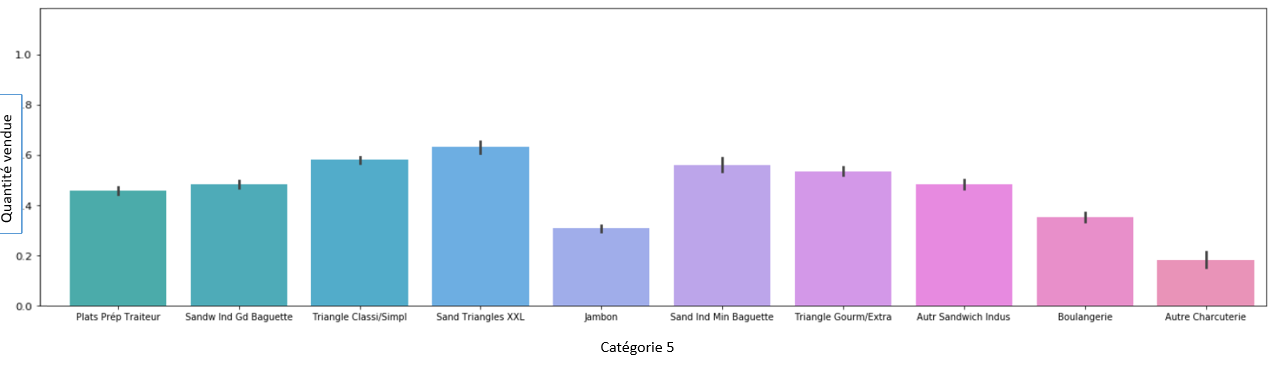
\includegraphics[keepaspectratio = true,scale=0.65]{categorie5part2.png}
	\caption{Ventes cumulées en fonction de la catégorie 5 (partie 2)}
	\label{fig:cat5p2}
\end{figure}
\subsection{Transformation des données}
\subsubsection{One Hot Encoding}
Le One Hot Encoding est une transformation des données catégorielles en vecteur binaire. La \textbf{Figure ~\ref{fig:OHE}} représente une telle transformation.
\begin{figure}[!h]
	\centering
	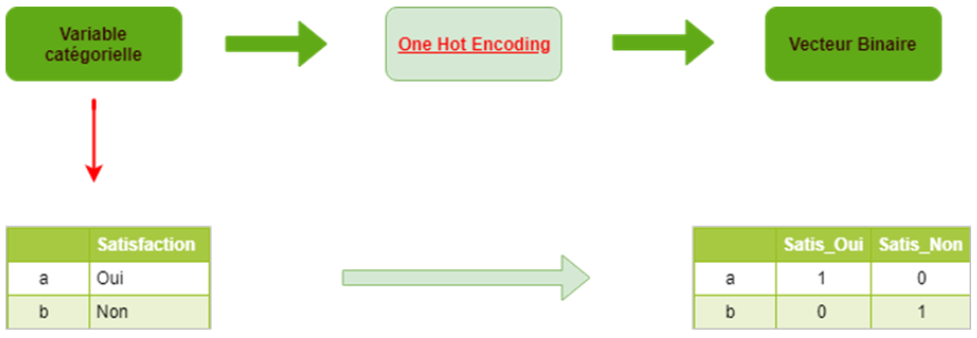
\includegraphics[keepaspectratio = true,scale=0.55]{OHE.png}
	\caption{Principe du One Hot Encoding}
	\label{fig:OHE}
\end{figure}
Le principe est de créer un ensemble de nouvelles variables représentant une variable catégorielle (une variable par possibilité différente) prenant des valeurs binaires (0 ou 1). Il est important de faire cette transformation car plusieurs algorithme de machine learning n'arrivent pas à travailler avec les variables catégorielles. En l'occurrence, concernant notre projet les modèles suivants ne supportent pas les variables catégorielles: \begin{itemize}
	\item Modèle linéaire
	\item Réseau de Neurone
\end{itemize}
Cependant il y a plusieurs désavantage à cette technique:
\begin{itemize}
	\item L'augmentation du nombre de dimensions qui est la cause de la \textit{"curse of dimensionality"}. Le traitement de données devient plus difficile et long, car les données prennent plus de place en mémoire
	\item Les éléments du vecteurs sont équidistants, impliquant que chaque modalité d'une variable catégorielle ait la même importance ce qui n'est pas le cas. (Par exemple, le fait qu'il y a des vacances en zone A, B et C est plus important que le fait qu'il n'y ait pas de vacances).
	\item Le vecteur binaire contient une information sémantique encodée, ce qui rend plus difficile la compréhension.
\end{itemize}
Cette méthode étant simple à appliquer et permettant l'utilisation directe de la majorité des algorithme, nous allons l'utiliser pour tous nos modèles dans la suite du projet.
 
\subsubsection{Normalisation des données}
De même que pour le One Hot Encoding, il est nécessaire (ou préférable) pour certains algorithmes, en particulier le Réseau de Neurones, d'avoir des données normalisées. En effet le Réseau de Neurones ne prend en entrée que des données normalisées. Nous avons donc normalisé par rapport à la différence minimum/ maximum pour chaque variable numérique.\\
La normalisation permet aussi d'avoir une convergence plus rapide pour les algorithmes basés sur de l'optimisation par gradient (Gradient boosting). Ce dernier se base sur une step size (le gradient de la fonction d'erreur multiplié par le taux d'apprentissage), cependant si les variables ne sont pas sur la même échelle, les step sizes sont différentes (car le gradient est différent), rendant la méthode de gradient boosting plus longue.\\
De plus elle permet d'avoir de meilleurs résultats pour le modèle linéaire, car celui-ci est moins affecté par les grandes variations. Les variables ayant un grand intervalle de définition vont induire une grande variance au modèle, ce qui leur donne trop d'importance.\\
Pour toute ces raisons, nous appliquons une normalisation des données.
\newpage
\section{Modélisation}
\alertinfo{Le code lié à cette partie est disponible sur le lien suivant \url{https://github.com/Syndorik/ChallengeTotal/blob/master/Data-Engineering-and_Modeling.ipynb}. 
}
Dans cette section, nous présentons l'ensemble des modèles qui ont été testés pour modéliser le problème posé par Argedis. 
\subsection{Modélisation basée sur le Data Engineering}
Le modèle doit répondre à un problème de régression de machine learning supervisé. Ici, on considère la variable comme continue (classement supervisé), bien qu'elle soit en réalité discontinue. En effet, comme précisé en Introduction, la quantité vendue d'un produit est le multiple d'un certain nombre propre au produit. Ainsi dans l'idéal, un modèle aurait été développé par produit. Dans ce cas là, le problème aurait été un problème de classification. Cependant, au vu de la faible taille de notre jeu de données, il peut être compliqué de faire un modèle par produit. On a choisi de garder comme base d'entraînement l'ensemble des produits.\\
Une autre possibilité aurait été de faire un modèle apprenant sur les périodes de travail (hors vacances) et un modèle apprenant sur les vacances. Comme nous l'avons vu, les périodes de vacances sont anormales : périodes de haute variance de quantité d'articles vendues. Donc cela va avoir tendance à perturber les modèles. Cependant nous n'avions qu'une année et demi de données. La période trop courte pour pouvoir faire cela. Il est à noter que les Time Series vont nous aider sur cette problématique. 
Nous allons détailler l'ensemble des modèles suivant :
\begin{itemize}
	\item Régression linéaire
	\item Decision Tree Regressor
	\item Extra Tree Regressor
	\item Random Forest Regressor
	\item Gradient Boosting Regressor
	\item XGBOOST
	\item Multi-layer Perceptron (MLP)
\end{itemize}

\subsubsection{Méthodologie d'évaluation des modèles}
Comme nous l'avons énoncé en Introduction, notre modèle est évalué selon le RMSE : 
$\sqrt{\frac{\sum_{i=1}^{n}(\hat{y}_t-y_t)^2}{n}}$. La méthode que nous avons utilisé pour s'assurer de la validité d'un modèle est la validation croisée (cross-validation). Le principe est d'entraîner le modèle sur une partie du jeu de données, 80\% par exemple et d'utiliser les 20\% restant pour le tester. Le processus est répété un nombre n de fois, et la moyenne des scores RMSE obtenus nous permet d'évaluer le modèle

\subsubsection{Méthodologie d'amélioration des modèles}
Chaque modèle, que nous allons expliciter dans les parties suivantes, possède des paramètres qui lui sont propre. Pour chaque modèle nous allons énoncer les paramètres les plus important. Cependant la méthodologie pour optimiser ces derniers est la même. Pour chaque combinaison de paramètre, nous allons lancer l'apprentissage d'un modèle et son évaluation par cross-validation (en RMSE).\\
Les paramètres du modèle ayant la meilleure évaluation seront considérés comme optimum. Dans la pratique, il existe une multitude de paramètres pour chaque algorithme, en général nous n'appliquons cette méthode que pour certains d'entre eux.


\subsubsection{Régression linéaire}
Ce modèle essaie de décrire les relations entre la variable à prédire et les variables d'entraînement comme linéaire (du type : $Y = \beta_0 + \beta_1X_1 + \beta_2X_2 ...$ avec $Y$ la variable à prédire et les $X_i$ les variables d'entraînements). La méthode utilisée pour créer la courbe de régression est la méthode des moindres carrés. On obtient après entraînement un score $R^2$ de 35.4\%, ce qui veut dire que ce modèle explique 35.4\% de la variance. Le score RMSE est le suivant
\alertinfo{RMSE = 0.9568 }
Ce score est assez faible surtout en comparaison des autres modèles. Cela est assez logique, car les relations au sein de notre jeu de données ne sont clairement pas linéaires, et il est assez difficile de modéliser des relations non linéaires avec ce modèle. C'est possible via l'introduction de termes d'interaction, mais cela reste assez primaire comme modélisation.

\subsubsection{Decision Tree Regressor et Extra Tree Regressor}
Ces modèles se basent sur la création d'arbres afin de fournir une prédiction. Le principe est que chaque feuille de l'arbre de décision va utiliser une variable pour effectuer une partition des données. Les arbres de décision permettent d'avoir un modèle qui est compréhensible en sortie d'apprentissage. Nous obtenons les résultats suivant :
\alertinfo{$RMSE_{Decision-tree-Regressor} = 0.669$ et $RMSE_{Extra-tree-regressor} = 0.646$ }
La différence entre le Decision Tree Regressor et l'Extra Tree Regressor repose sur la manière séparer la population au sein d'un noeud afin de créer une branche. L'Extra Tree Regressor va prendre un certain nombre de variables au sein d'un noeud, regarder quelle est la meilleure manière de séparer le noeud à partir de ces variables et recommencer le processus plusieurs fois. Le meilleur \textit{split} est alors choisi.\\
Cela explique pourquoi l'Extra Tree Regressor possède un meilleur score RMSE. Cependant, le grand inconvénient de ces méthodes est qu'elles ont tendance à sur-apprendre ou au contraire pas assez apprendre en fonction de la profondeur de l'arbre. C'est pourquoi nous nous sommes concentrés sur les modèles ensemblistes d'arbre de décision.\\
Paramètres principaux à optimiser : la profondeur de l'arbre, le nombre minimum de feuilles

\subsubsection{Random Forest Regressor}
Les forêts d'arbres de décision ou random forest, se basent sur la création de plusieurs arbres de décision. Le principe est de créer plusieurs arbres de décision de manière aléatoire : sélection aléatoire des variable et du jeu d'apprentissage (bootstrap sample). Une fois l'apprentissage des arbres fini, il suffit de moyenner la sortie de chaque arbre de décision pour obtenir la variable à prédire. C'est le principe du bagging.Nous obtenons les résultats suivants :
\alertinfo{$RMSE = 0.57997$ }
Le score obtenu est meilleur que pour les précédents modèles utilisés. Cela s'explique par l'aspect général du modèle qui permet de compenser les problèmes de sur-apprentissage que l'on peut rencontrer avec un arbre de décision unique. L'inconvénient de cette méthode est le temps d'exécution qui peut être assez long.\\
Paramètres principaux à optimiser : la profondeur de l'arbre, le nombre minimum de feuilles, le nombre d'arbres maximum.

\subsubsection{Gradient Boosting et XGBOOST Regressor}
Ces deux modèles sont des versions modifiées des forêts d'arbres de décision. Au lieu de se baser sur du bagging pour créer les arbres de décisions, ils se basent sur des méthodes de gradient boosting. Le principe est de créer des arbres de décisions à la chaîne. Cependant entre chaque création d'arbre, l'erreur est minimisée en utilisant la méthode de descente du gradient. Nous obtenons les résultats suivant :
\alertinfo{$RMSE = 0.57909$ }
Le score obtenu est meilleur que pour les forêts d'arbres aléatoires. Cependant, la différence se fait au millième du RMSE. Sachant que notre prédiction est continue alors que la quantité vendue par produit prend des valeurs discontinue, la différence obtenue n'est pas significative. En effet l'erreur due à l'échantillonnage est plus grande.\\
On peut trouver une explication à ces résultats par le fait que les deux algorithmes reposent sur la création d'arbres de décision. Les forêts d'arbres aléatoires vont en général essayer de réduire la variance tandis que les méthodes de boosting vont essayer de réduire le biais. Ici, il apparaît que dans les deux cas nous obtenons une erreur similaire.\\
Paramètres principaux à optimiser : le taux d'apprentissage, la profondeur de l'arbre, le nombre minimum de feuilles, le nombre d'arbres maximum.

\subsubsection{Multi-layer Perceptron (MLP)}
Cet algorithme repose sur la création d'un réseau de neurones. Il va apprendre une fonction à partir du jeu de données. L'avantage est la capacité de modéliser les non linéarités. Le réseau de neurones comporte 4 couches dont deux cachées. La première est l'input layer, la seconde est composée de 32 neurones, la deuxième de 16 neurones, et la dernière de un neurone (correspondant à la variable à prédire). La fonction d'activation utilisée est la fonction "relu". 
\alertinfo{$RMSE = 0.685$ }
Le score obtenu est moins bon que pour les autres modèles testés auparavant. Cela est probablement dû au fait que notre réseau de neurones n'est pas adapté à notre problème et qu'il pourrait être optimisé. Cependant le temps d'apprentissage du réseau étant relativement long, nous n'avons pas insisté sur cette voie. 

\subsubsection{Stacking}
Cette méthode ensembliste permet de combiner les meilleurs modèles précédemment créés afin d'obtenir un modèle plus performant. Dans notre cas, nous avons pris 3 modèles différents, le modèle linéaire, le modèle de forêts aléatoire et le modèle Gradient Boosting. Le principe est décrit en \textbf{Figure ~\ref{fig:stacking}}. Le jeu de données est divisé en différentes bases d'apprentissages pour différents modèles. Les prédictions faites à partir des modèles vont ensuite servir de base d'apprentissage au meta-modèle. Dans notre cas ce sera un XGBOOST. Nous obtenons alors le résultat suivant : 
\alertinfo{$RMSE = 0.5735$ }
Le score obtenu est meilleur mais ne varie que de quelques centièmes. En effet, le stacking est utile pour combiner des modèles qui ont des zones d'erreurs assez différentes. Les modèles basés sur les forêts d'arbres de décision et les modèles basés sur XGBOOST ont des zones d'erreurs assez similaires. Ainsi, nos modèles sont trop similaires pour bénéficier du stacking.

\begin{figure}[!h]
	\centering
	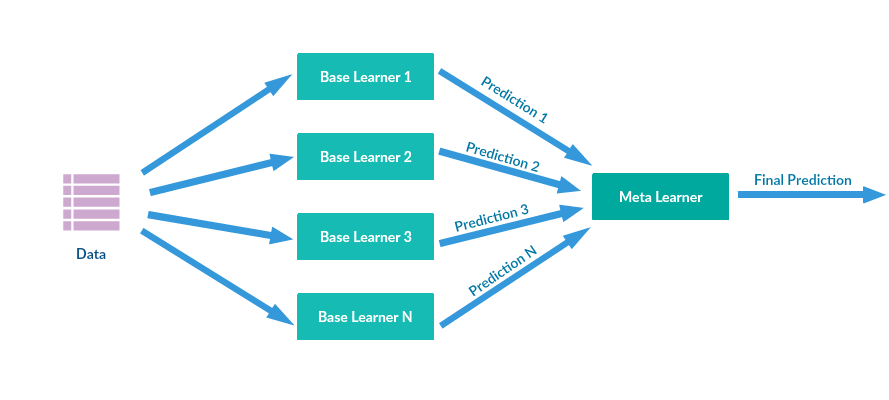
\includegraphics[keepaspectratio = true,scale=0.65]{stacking.png}
	\caption{Principe du stacking}
	\label{fig:stacking}
\end{figure}
\newpage
\subsubsection{Post-traitement}
Nous avons implémenté deux post-traitements en vue d'améliorer la qualité de notre modèle.
\begin{itemize}
	\item Il existe des produits qui étaient disponibles dans une station mais pas dans l'autre, et vice-versa. Nous savons dès lors, que s'il est demandé de prédire le nombre de vente d'un produit qui n'existe pas dans la station, il sera prédit automatiquement à 0.
	\item Nous savons qu'un produit ne peut prendre comme valeurs de quantité vendue que des multiples d'une quantité de base. Cette quantité de base est différente pour chaque produit. Ainsi, nous avons tenté d'approximer chaque quantité vendue, soit par sa valeur de multiple supérieure, soit par sa valeur de multiple inférieure. 
\end{itemize}
Le premier point du post-traitement est assez efficace et améliore effectivement les prédictions des modèles.\\
Le deuxième point est bien plus problématique. Nous l'avons testé  sur les résultats du modèle stacké et nous sommes passés d'un RMSE de 0.5735 à un RMSE de 0.72. Nous nous attendions à une régression légère du score RMSE, cependant ici cela est bien trop grand. Il y a plusieurs explications possibles. Tout d'abord, notre post-traitement se trompe pour chaque produit et retourne toujours la mauvaise valeur (ie il retourne la valeur au-dessus quand la valeur réelle est en-dessous et inversement). Cette première explication semble assez improbable. Une seconde explication serait une mauvaise compréhension de la variable quantité vendue. En effet, aucune information dans le jeu de données ne nous dit ce qu'elle représente exactement.


\subsection{Modélisation basée sur les Time Series}
\label{sec:tm}
\alertinfo{Le code lié à cette partie est disponible sur le lien suivant \url{https://github.com/Syndorik/ChallengeTotal/blob/master/Time_series.ipynb}. 
}


\newpage
\subsection{Analyse des résultats}
Etudes par produit aurait pu être plus fructueuse. Cela n'a pas été fait, mais peut donner des meilleurs résultats, surtout que les ventes de produits sont très différentes et varie différement. 
\newpage
\section{Conclusion}

\newpage
\section{Annexe}
\subsection{Vente par Catégorie de produit}
\label{sec:catprod}
\begin{figure}[!h]
	\centering
	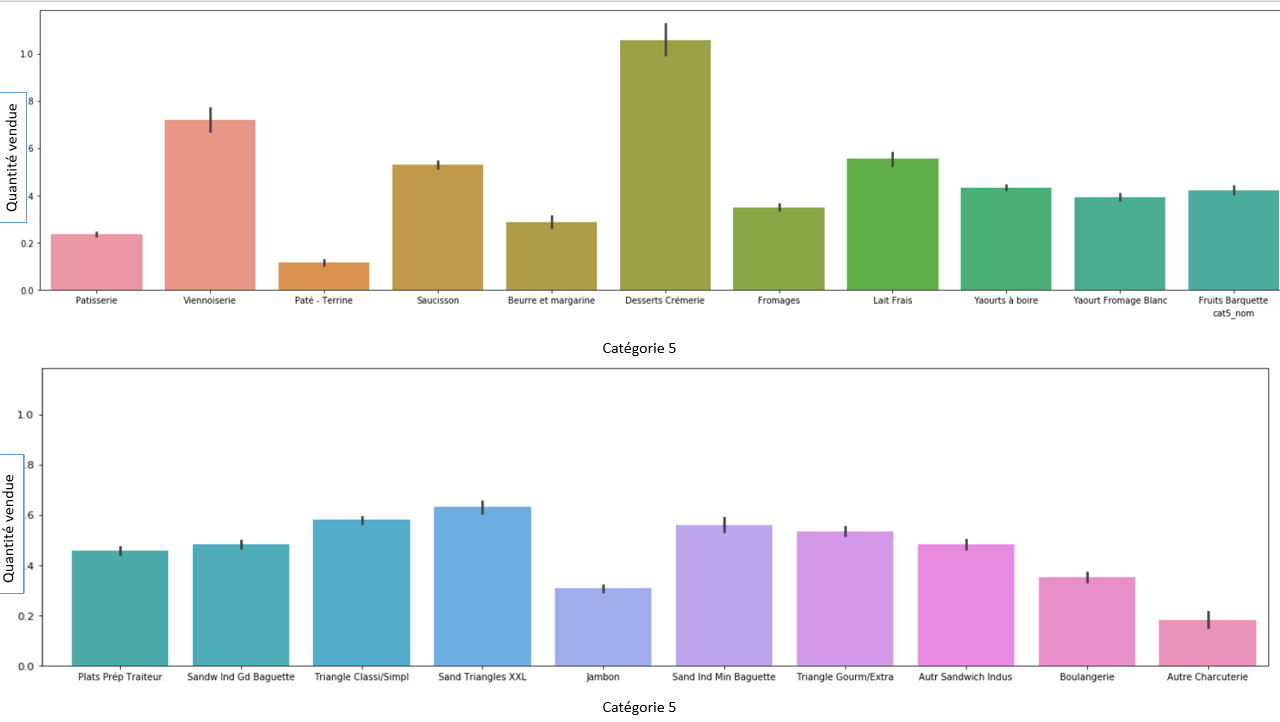
\includegraphics[keepaspectratio = true,scale=0.65]{categorie.png}
	\caption{Vente cumulé en fonction de la catégorie 5}
\end{figure}

\begin{figure}[!h]
	\centering 
	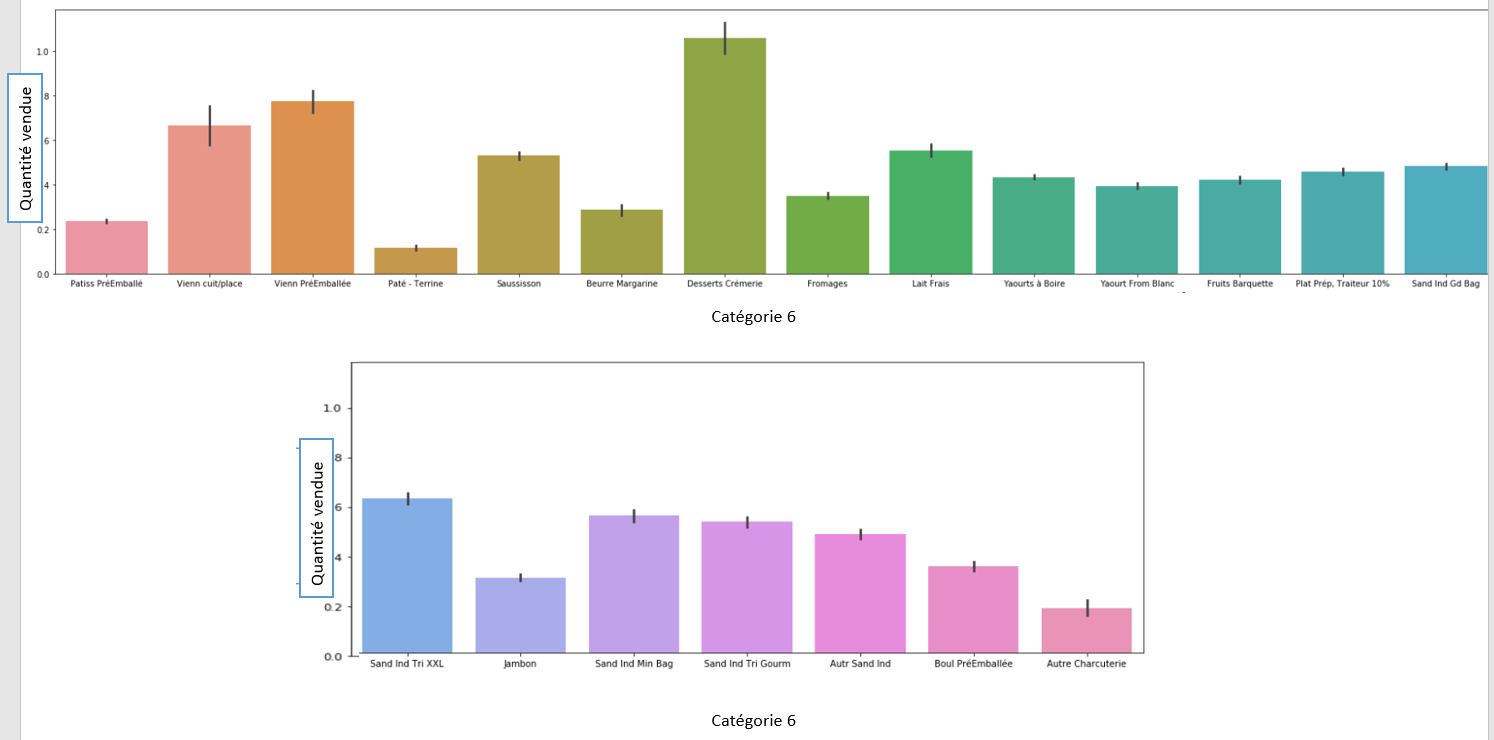
\includegraphics[keepaspectratio = true,scale=0.55]{categorie6.png}
	\caption{Vente cumulé en fonction de la catégorie 6}
	\label{bb3}
\end{figure}
\newpage
\begin{figure}[!h]
	\centering
	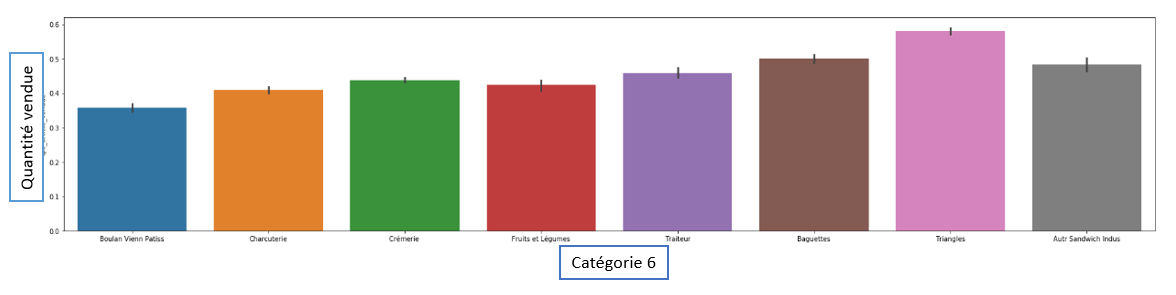
\includegraphics[keepaspectratio = true,scale=0.55]{categorie4.png}
	\caption{Vente cumulé en fonction de la catégorie 4}
	\label{bb3}
\end{figure}
\end{document}
%%%%%%%%%% END %%%%%%%%%% 
%%%%%%%%%%%%%%%%%%%%%%%%% 
